\documentclass[11pt, oneside]{article}   	% use "amsart" instead of "article" for AMSLaTeX format
\usepackage{geometry}                		% See geometry.pdf to learn the layout options. There are lots.
\geometry{letterpaper}                   		% ... or a4paper or a5paper or ... 
%\geometry{landscape}                		% Activate for for rotated page geometry
%\usepackage[parfill]{parskip}    		% Activate to begin paragraphs with an empty line rather than an indent
\usepackage{graphicx}				% Use pdf, png, jpg, or eps� with pdflatex; use eps in DVI mode
								% TeX will automatically convert eps --> pdf in pdflatex		
\usepackage{amssymb}
\usepackage{amsmath}
\usepackage{parskip}
\usepackage{color}
\usepackage{hyperref}

\title{Power series}
%\author{The Author}
%\section{}
%\subsection*{}
\date{}							% Activate to display a given date or no date

\graphicspath{{/Users/telliott_admin/Dropbox/Tex/png/}}
% \begin{center} 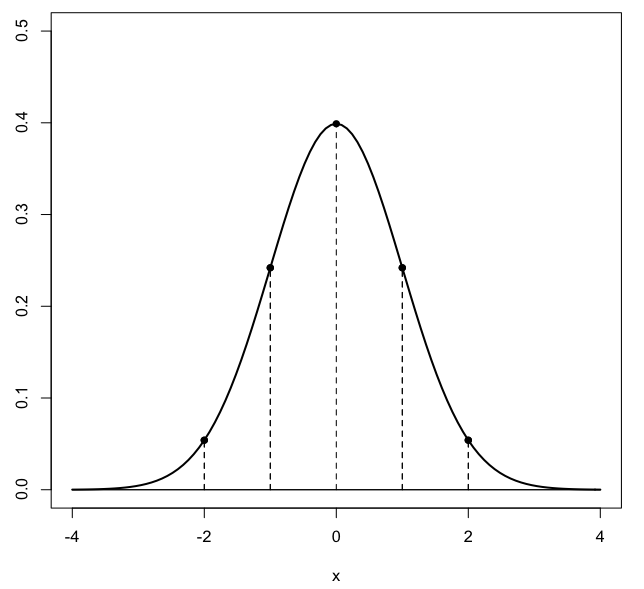
\includegraphics [scale=0.4] {gauss3.png} \end{center}
\begin{document}
\maketitle
\Large
\[ f(z) = \sum_0^{\infty} a_n \ (z-z_0)^n \]
If $f(z)$ has a positive (or infinite) radius of convergence, then inside the disk $|z-z_0| < R$, $f(z)$ is infinitely differentiable, and each derivative is given by a power series:
\[ f^{(k)}(z) = \sum_{n=k}^{\infty} n(n-1) \dots (n-k+1) \ a_n \ (z-z_0)^{n-k} \]
Consider as an example this power series with $a_n = n$:
\[ f(z) = \sum_0^{\infty} n \ z^n = 0 + z + 2z^2 + 3z^3 \dots \]
Differentiate term by term:
\[ f'(z) = 1 + 2^2 z + 3^2 z^2 + \dots + n^2 z^{n-1} + \dots \]
Does this match the definition?
\[ f^{(k)}(z) = \sum_{n=k}^{\infty} n(n-1) \dots (n-k+1) \ a_n \ (z-z_0)^{n-k} \]
The first derivative is for $k=1$ so
\[ n \dots (n-k+1) = n \]
and $z_0 = 0$ so
\[ f'(z) = \sum_{n=1}^{\infty}n \ a_n \ z^{n-1} \]
Recall that $a_n = n$
\[ = \sum_{n=1}^{\infty}n^2 \ z^{n-1} \]
which indeed matches
\[ f'(z) = 1 + 2^2 z + 3^2 z^2 + \dots + n^2 z^{n-1} + \dots \]

Go back to 
\[ f^{(k)}(z) = \sum_{n=k}^{\infty} n(n-1) \dots (n-k+1) \ a_n \ (z-z_0)^{n-k} \]
If $z = z_0$ then
\[ f^{(k)}(z_0) = \sum_{n=k}^{\infty} n(n-1) \dots (n-k+1) \ a_n \ 0^{n-k} \]
Now you might think that all these terms would be zero, and they are provided that $n-k \ne 0$, but there:
\[ f^{(k)}(z_0) = \sum_{n=k}^{\infty} n(n-1) \dots 1 \ a_n \ 0^{0} \]
\[ f^{(k)}(z_0) = n! \ a_n\]
\[ a_n = \frac{1}{n!} \ f^{(k)}(z_0)  \]
And the reason is that 
\[ 0^0 = \lim_{n \rightarrow 0} n^n = 1 \]
\url{http://mathforum.org/dr.math/faq/faq.0.to.0.power.html}

\subsection*{exponential}
Write the exponential as
\[ e^z = \sum_{n=0}^{\infty} \frac{z^n}{n!} = 1 + z + \frac{z^2}{2} + \frac{z^3}{3} + \dots \]
We could use the formula for the derivative, or just differentiate term by term and obtain that
\[ f(z) = f'(z) \]
Now write (by the chain rule)
\[ \ [ \ e^{-z} f(z) ] ' = -e^{-z} f(z) + e^{-z} f'(z) \]
and since $f(z) = f'(z)$
\[ = -e^{-z} f'(z) + e^{-z} f'(z) \]
But this is just 0.  So that means the original compound function is a constant, since its derivative is zero:
\[ e^{-z} f(z) = C \]
and this is true for any $z$ so
\[ e^0 f(0) = f(0) = C \]
so going back to the series, when $z=0$
\[ f(0) = \sum_{n=0}^{\infty} \frac{z^n}{n!} = \sum_{n=0}^{\infty} \frac{0^n}{n!} \]
Now, the numerator is zero for all terms except $n=0$ where it is equal to $1$ (see above), and that denominator is $0! = 1$, so 
\[ f(0) = 1 = C \]
Thus
\[ e^{-z} f(z) = 1 \]
\[ f(z) = e^z \]

\end{document} 